\documentclass[12pt]{article}
\usepackage[utf8]{inputenc}


%\pagenumbering{Roman}
%\renewcommand\thepage{\arabic{page}}
\usepackage{ragged2e}
\usepackage{graphicx,float}
\usepackage{wrapfig}
\usepackage{hyperref}
\usepackage[margin=1in]{geometry}
\usepackage{subcaption}
% \usepackage{subfigure}
\usepackage{xcolor}
\usepackage{tikz}
%\usepackage{amssymb}
%\usepackage{makecell}
\usepackage{multirow}
%\usepackage{boldline} 
\usepackage{array}
\usepackage{booktabs}
\usepackage{siunitx}
\usepackage{cite}
\usepackage{setspace}
\usepackage[nottoc,notlot]{tocbibind}

\usepackage{blindtext}

\setlength{\parskip}{1em}
\usepackage[most]{tcolorbox}

\graphicspath{ {images/} }
\usepackage{titling}

\newcommand{\proposalTitle}{Spherical Normalization, Differential Encoding, and Complex-valued Convolutions for Deep Learning in Time-varying MIMO Channel State Estimation}
\newcommand{\authorName}{Mason del Rosario}
\newcommand{\authorDepartment}{Electrical and Computer Engineering}
\newcommand{\authorUniversity}{University of California, Davis}
\newcommand{\authorAddress}{Davis, CA 95616}
\newcommand{\authorEmail}{mdelrosa@ucdavis.edu}

\title{}

\author{
	\authorName\\
	%  <Department> of Electrical and Computer Engineering\\
	\authorDepartment\\
	\authorAddress \\ % in US, this will be <City>, <State> <ZIP> for University
	\authorEmail \\
}

\date{\today}

\doublespacing

\begin{document}
	
% 00_title.tex

\begin{titlepage}
	\null\vfill
	
	\begin{center}
		
		{\Huge \proposalTitle}
		\vskip 2cm
		
		{\Large \authorName}
		\vskip 1cm
		
		{\large \authorUniversity\\
				\authorAddress \\
				\texttt{\authorEmail} \\}
	\end{center}
	
	\vfill
	\vfill
	
	\centering
	\begin{tabular}{r}
		\today \\
	\end{tabular}
\end{titlepage}



\newpage
\tableofcontents

\newpage

\section{Introduction}
% 01_introduction.tex

% Section \ref{sect:notation} introduces the notation used through this work.
This qualifying examination proposal details work in improving the accuracy and efficiency of deep learning methods for MIMO channel state information estimation. Section \ref{sect:mimo_model} provides an overview of the MIMO channel. Section \ref{sect:channel_model} introduces the channel simulation used in this work, the COST2100 model. Section \ref{sect:classic_estimation} discusses prior work in compressed sensing for CSI estimation. Section \ref{sect:dl_overview} provides a generic overview of deep learning. 
Boldface lowercase (uppercase) letters indicate vectors (matrices). Unless otherwise specified, the norm $\|\cdot\|$ indicates the Frobenius norm. Superscripts $^T$ ($^H$) indicate the transpose (Hermitian transpose).
% recent work in deep learning for CSI estimation in MIMO networks

\section{MIMO Channel Overview}
\label{sect:mimo_model}

\begin{figure}[!hbtp]
\centering
{
	\fontsize{6pt}{8pt}
	\def\svgwidth{0.8\columnwidth}
	\input{../images/mimo-schematic.pdf_tex}
}
\caption{Example multi-antenna transmitter (BS, gNB) and single-antenna user equipment (UE) and relevant system values.}
\label{fig:mimo_schematic}
\end{figure}

In this work, we consider a MIMO channel with a multiple antennas ($N_B \gg 1$) at the transmitter (gNodeB or gNB) servicing a single user equipment (UE) with a single antenna. Under orthogonal frequency division multiplexing (OFDM) with $N_f$ subcarriers, the received symbols on the $m$-th subcarrier for the downlink and the uplink at the receiver are given as
\begin{align*}
	y_{d,m} &= \mathbf h_{d,m}^H\mathbf w_{t,m}x_{d,m} + n_{d,m}.
	% y_{u,m} &= \mathbf w_{r,m}^H\mathbf h_{u,m}x_{u,m} + \mathbf w_{r,m}^H\mathbf n_{u,m},
\end{align*}
where the individual system values are defined in Table~\ref{tab:mimo-params}, and a representative system model is viewable in Figure~\ref{fig:mimo_schematic}. The resulting downlink and uplink channel state information (CSI) matrices are given as
\begin{align*} 
	\bar{\mathbf H}_d &= \begin{bmatrix} \mathbf h_{d,1} & \dots & \mathbf h_{d,N_f}\end{bmatrix}^H \in \mathbb C^{N_f \times N_b}.
	% \bar{\mathbf H}_u &= \begin{bmatrix} \mathbf h_{u,1} & \dots & \mathbf h_{u,N_f}\end{bmatrix}^H \in \mathbb C^{N_f \times N_b}.
\end{align*}
\begin{table}[]
\renewcommand{\arraystretch}{1.25}
\centering
\caption{MIMO system variables considered in this work.}
\label{tab:mimo-params}
\begin{tabular}{c|c|l}
\toprule
\textbf{Symbol}   	  	  & \textbf{Dimension}            & \textbf{Description} \\ \midrule
$y_{d,m}$ 		  	  	  & $\mathbb{C}^{1}$ 			  & Received downlink symbol on $m$-th subcarrier  \\ \hline
$\mathbf h_{d,m}$ 	  	  & $\mathbb{C}^{N_b \times 1}$   & Downlink channel on $m$-th subcarrier  \\ \hline
$\bar{\mathbf H}_{d}$ 	  & $\mathbb{C}^{N_f \times N_b}$ & Downlink CSI (spatial-frequency domain)  \\ \hline
$\mathbf w_{t,m}$ 	  	  & $\mathbb{C}^{N_b \times 1}$   & Transmitter precoding vector for $m$-th subcarrier  \\ \hline
$x_{d,m}$ 		  	  	  & $\mathbb{C}^{1}$ 			  & Trasmitted symbol on $m$-th subcarrier  \\ \hline
$n_{d,m}$ 		  	  	  & $\mathbb{C}^{1}$ 			  & Downlink noise on $m$-th subcarrier  \\ \hline
$\tilde{\mathbf H}_{d}$   & $\mathbb{C}^{N_f \times N_b}$ & Downlink CSI (angular-delay domain)  \\ \hline
$\mathbf H_{d}$   		  & $\mathbb{C}^{R_d \times N_b}$ & Truncated downlink CSI (angular-delay domain)  \\ \hline
% $y_{u,m}$ 		  & $\mathbb{C}^{1}$ 			  & Received uplink symbol on $m$-th subcarrier  \\ \hline
% $\mathbf h_{u,m}$ & $\mathbb{C}^{N_b \times 1}$   & Uplink channel on $m$-th subcarrier  \\ \hline
% $\mathbf H_{u}$   & $\mathbb{C}^{N_f \times N_b}$ & Downlink impulse response on $m$-th subcarrier  \\ \hline
% $\mathbf w_{r,m}$ & $\mathbb{C}^{N_b \times 1}$   & Received precoding vector for $m$-th subcarrier  \\ \hline
% $x_{u,m}$ 		  & $\mathbb{C}^{1}$ 			  & Received symbol on $m$-th subcarrier  \\ \hline
% $\mathbf n_{u,m}$ & $\mathbb{C}^{1}$ 			  & Uplink noise on $m$-th subcarrier  \\ \hline
\end{tabular}
\end{table}
To achieve near-capacity transmission rates, the transmitter needs access to an appropriate estimate of $\bar{\mathbf H}_d$ \cite{ref:goldsmith2003capacity}. Such estimates enable the use of linear precoding techniques (e.g., conjugate beamforming or zero-forcing beamforming) to realize appreciable spectral and power efficiency gains \cite{ref:yang2013performance}. Downlink CSI estimation can be performed in time division duplex (TDD) by using uplink pilots due to channel reciprocity \cite{ref:Kaltenberger2010relative,ref:mi2017massive,ref:Gao2010utilization}. In contrast, frequency domain duplex (FDD) does not admit channel reciprocity due to frequency-selective channels, and CSI estimates must be acquired using feedback.



\section{Channel Model}
\label{sect:channel_model}

For all CSI tests, we mainly rely on the COST2100 MIMO channel model \cite{ref:liu2012cost2100}. We use two datasets with a single base station (gNB) and a single user equipment (UE) in the following scenarios:
\begin{enumerate}
	\item \textbf{Indoor} channels using a 5.3GHz downlink at
	0.001 m/s UE velocity, served by a
	gNB at center of a $20$m$\times 20$m coverage area.
	\item \textbf{Outdoor} channels using a 300MHz downlink at 0.9 m/s UE velocity served by a gNB at center 
	of a $400$m$\times 400$m coverage area.
\end{enumerate}
In both scenarios, we use the parameters listed in Table~\ref{tab:cost-params}.
\begin{table}[]
\centering
\caption{Parameters used for COST2100 simulations for both Indoor and Outdoor datasets.}
\label{tab:cost-params}
\begin{tabular}{c|c|l}
\toprule
\textbf{Symbol} & \textbf{Value} & \textbf{Description} \\ \midrule
$N_b$ 			& 32			 & Number of antennas at gNB  \\ \hline
$N_f$ 			& 1024			 & Number of subcarriers for OFDM link  \\ \hline
$R_d$ 			& 32			 & Number of delay elements kept after truncation  \\ \hline
$N$ 			& $10^6$		 & Total number of samples per dataset  \\ \hline
$T$ 			& 10		 	 & Number of timeslots  \\ \hline
$\delta$		& 40 ms			 & Feedback delay interval between consecutive CSI timeslots  \\ \bottomrule
\end{tabular}
\end{table}

\section{Classical CSI Estimation}
\label{sect:classic_estimation}

Works in compressive feedback for CSI estimation in MIMO networks can be placed in three broad categories. The first category includes works which use direct quantization of continuous CSI elements to discrete levels. The quantized CSI are encoded and fed back to the transmitter \cite{ref:makki2012hybrid,ref:shirani2009channel}. The second category includes works which use compressed sensing, a technique which applies a random measurement matrix at the transmitter and the receiver \cite{ref:rao2014distributed, ref:eltayeb2014compressive}. Compressed sensing assumes matrices to be encoded and fed back meet certain sparsity requirements, and compressed sensing algorithms require iterative solvers \cite{ref:do2008sparsity} for decoding, resulting in undesired latency.

The last category of work in compressive CSI feedback uses deep learning (DL), neural networks with numerous layers which are trained on large datasets using backpropagation. Before describing these works, we first describe a few pertinent concepts from deep learning.

\section{Deep Learning Background}
\label{sect:dl_overview}

This section provides a brief overview of relevant deep learning concepts employed in this work, including convolutional neural networks (CNNs), autoencoders, and unsupervised learning.

\textbf{Deep learning (DL)} is a subset of machine learning (ML), a broad class of algorithms which use data to ``fit'' models for prediction or classification tasks. The three predominant learning frameworks are supervised learning, unsupervised learning, and reinforcement learning. In the works proposed, we focus on \emph{unsupervised learning}, which seeks to find a compressed representation of the data without labels (see Chapter 14 of \cite{ref:Hastie2016Elements} for an overview).

\textbf{Convolutional Neural Networks}: A neural network is a machine learning algorithm with multiple \emph{layers} of parameterized linear functions followed nonlinear functions (typically referred to as `activation' functions). The parameters for these layers can be updated via a stochastic optimizer (e.g., \cite{ref:Kingma2014ADAM}), and given enough layers, such networks can achieve arbitrarily accurate functional approximation \cite{ref:Hecht1992TheoryBackprop}. In recent years, neural networks with convolutional layers have established state-of-the-art performance in computer vision tasks such as image classification \cite{ref:Sabour2017Dynamic} and segmentation \cite{ref:He2017Mask}.

\begin{figure}[!hbtp]
\centering
\def\svgwidth{0.8\columnwidth}
\input{../images/autoencoder_schematic.pdf_tex}
\caption{Abstract schematic for an autoencoder operating on CSI matrices $\mathbf H$. The encoder learns a latent representation, $\mathbf Z$, while the decoder learns to reconstruct estimates $\hat{\mathbf H}$.}
\label{fig:autoencoder_schematic}
\end{figure}

A common architecture for deep unsupervised learning is the \emph{autoencoder} (see Fig.~\ref{fig:autoencoder_schematic} for a generic example). Trained end-to-end on input data, an autoencoder is comprised of an encoder and a decoder which jointly learn a compressed latent representation ($\mathbf Z$) and an estimate of the input ($\hat{\mathbf H}$). By choosing $\mathbf Z$ to have lower dimension than the input, the network is forced to learn a ``useful'' summary of the input data. The typical objective function for such a network is the mean squared error (MSE),
\begin{align*}
\underset{\theta_e, \theta_d}{\text{argmin}}\; \frac 1N \sum_{i=1}^N\Arrowvert \mathbf H_i - g(f(\mathbf H_i, \theta_e), \theta_d) \Arrowvert^2.
\end{align*}
We optimize network parameters $\vec \theta_e, \vec \theta_d$ by backpropagation and a stochastic optimization algorithm (e.g., stochastic gradient descent, ADAM).

\section{Objective and Contributions}

Successful efforts in DL for CSI estimation have typically utilized convolutional neural networks (CNNs) in an autoencoder structure \cite{ref:csinet}. Variations on the CNN-based autoencoder have investigated different network architectures \cite{ref:Lu2020CRNet}, variational training frameworks \cite{ref:Hussien2020PRVNet}, and denoising modules \cite{ref:Sun2020AnciNet}. These architectural changes are largely inspired by successful application of DL in image compression \cite{ref:szegedy2017inception,ref:balle2017end,ref:xie2012image}.

While they can continue to push the state-of-the-art in CSI reconstruction accuracy, architectural optimizations may ultimately follow the same trends of fields such as language modeling, where state-of-the-art performance requires prohibitively massive compute \cite{ref:brown2020language}. In this proposal, we take a different approach seek to improving compressive channel feedback by focusing on domain knowledge and physical insight.
% While the powerful functional approximation of deep CNNs has enabled state-of-the-art CSI reconstruction accuracy, they run the risk falling into the same trap as the image.

This qualifying exam proposal details our attempts to use domain knowledge to enhance the performance and the efficiency of neural networks for CSI estimation (for a visual summary, see Figure~\ref{fig:contrib}). Section~\ref{chap:sph_norm} details our work in power-based normalization, which leverages CSI sparsity. Section ~\ref{chap:markovnet} describes our work in differential encoding, which exploits temporal coherence of CSI. Section~\ref{chap:csinet_quant} describes our proposed work in trainable codewords, which incorporates data-adaptive quantization in the training process, and CSI entropy estimation, which establishes a compression bound for deep learning-based compressive feedback of CSI.

\begin{figure}[htb] \centering 
	{
	  \fontsize{4pt}{4pt}
	  \def\svgwidth{0.9\columnwidth}
	  \input{../images/cnns-venn-diagram-contrib.pdf_tex}
	}
	\caption{Venn diagram highlighting different aspects of domain knowledge in CNN-based CSI compressive feedback, relevant convolutional networks, and our contributions.}
	\label{fig:contrib}
\end{figure}


\section{Spherical Normalization}
\label{chap:sph_norm}
% 02_previous_work_first.tex

Most work in deep learning for CSI estimation focuses on different neural network architectures, training frameworks, or hyperparameter tuning. However, the normalization used in these works is typically the same; the extrema (i.e., the minimum and the maximum) of the dataset are used to perform minmax scaling on the entire dataset, 
\begin{align*}
	\mathbf H_{k,\text{minmax}}(i,j) &= \frac{\mathbf H_k(i,j)-\mathbf H_{\text{min}}}{\mathbf H_{\text{max}}-\mathbf H_{\text{min}}}
\end{align*}
for $n \in [1,\dots,N]$ given a dataset of $N$ samples and $i,j$ indexing the rows/columns of the CSI matrices. The resulting samples are cast to the range $[0,1]$.

For image data, minmax normalization results in each image's color channels scaled to the range $[0,1]$. The resulting distribution for each color channel is typically satisfactory for image tasks, as the variance is not much smaller than the range of the normalized data (see Fig.~\ref{fig:imagenet_dist}).

However, for CSI matrices, minmax normalization is applied to the real and imaginary channels of each element. For typical channel models and parameters, the distribution of channel elements (see Fig.~\ref{fig:cost_indoor_dist}) tends to have much lower variance than that of ImageNet. This smaller variance can be explained by the difference in the datasets' ranges -- while the channels in image data (e.g., ImageNet) assume integer values between $[0,255]$, the channels in CSI data (e.g., COST2100) assume floating point values smaller than $10^{-3}$.

\begin{figure}[htb]
	\centering
	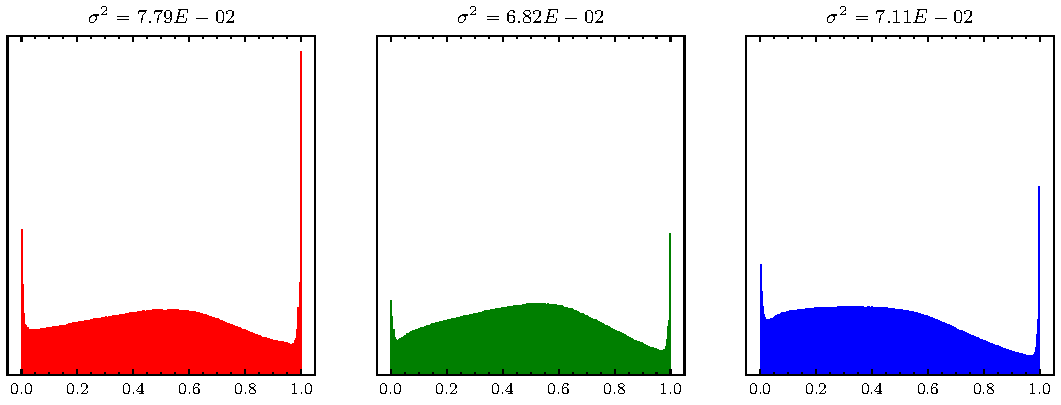
\includegraphics[width=.9\textwidth]{imagenet_rgb_dist.pdf}
	\medskip
	\caption{Distribution and variance of minmax-normalized ImageNet color channels ($N=50000$) images.}
	\label{fig:imagenet_dist}
\end{figure}

\begin{figure}[htb]
	\centering
	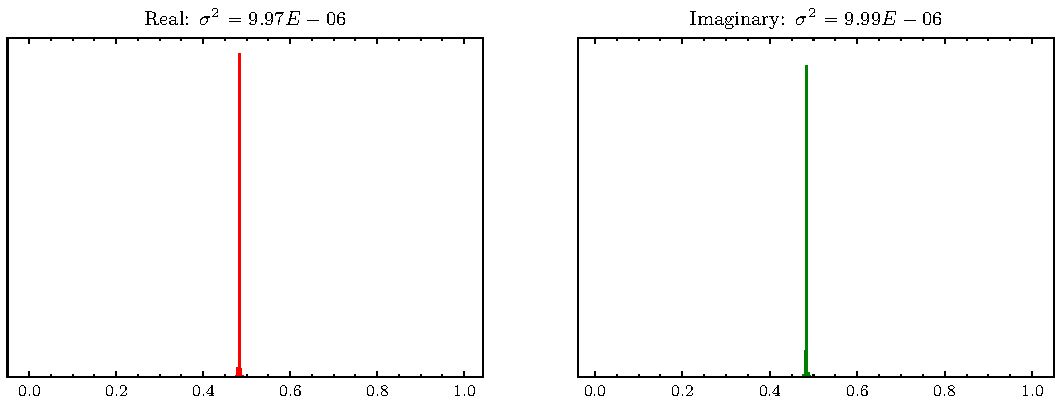
\includegraphics[width=.9\textwidth]{cost2100_indoor_dist.pdf}
	\medskip
	\caption{Distribution and variance of minmax-normalized COST2100 real/imaginary channels ($N=99000$) images.}
	\label{fig:cost_indoor_dist}
\end{figure}

\subsection{Related Work}

Several works have investigated normalization techniques for deep learning such as batch normalization \cite{ref:ioffe2015batch}, instance normalization \cite{ref:huang2017instance}, layer normalization \cite{ref:ba2016layer}, and group normalization \cite{ref:wu2018group}. These normalization techniques scale the outputs of latent layers in neural networks, which helps to solve the problem of covariate shift \cite{ref:ioffe2015batch} where the mean and variance of changes between subsequent layers of the network.

Other works have studied normalization of the network's inputs. A number of works have investigated adaptive normalization techniques for time series estimation tasks \cite{ref:ogasawara2010adaptive, ref:nayak2014impact, ref:shao2015self}. In \cite{ref:passalis2019dain}, the authors proposed a trainable input network which learns to shift, scale, and filter the unnormalized data while training the target network for a time series prediction task.

\subsubsection{Notation}

For an example of a table, see Table~\ref{table:notation}.

\begin{table}[htb]
	%	\small
	\caption{Notations}
	\label{table:notation}
	\centering
	\begin{tabular}[]{c|l}
		\toprule
		Variable & Definition \\
		\midrule
		$M$ & Number of input hydrological variables denoted in Fig.~\ref{fig:ann_inputs}\\
		\hline
		$N$ & Number of data samples, or days, in dataset \\
		\hline
		$T$ & Number of days' data used for estimation \\
		\hline
		$T_r$ & Dimension of data after pre-processing\\
		\hline
		$z_{n}$ & Time series used for estimating salinity level on day $n$, size is ${\rm I\!R}^{M\times T}$ \\
		\hline
		$x_{n}$ & Pre-processed time series with size ${\rm I\!R}^{M\times T_r}$ for day $n$\\
		\hline
		$f$ & A convolutional filter with size ${\rm I\!R}^{M \times T \times T_r}$ \\
		\hline
		$y_{n}$ & ANN-estimated salinity level for one or more locations on day $n$ \\
		\bottomrule
	\end{tabular}
\end{table}

% \begin{figure}[htb]
% 	\centering
% 	\includegraphics[width=.7\textwidth]{math_pipeline.png}
% 	\medskip
% 	\caption{Pipeline for ANNs in \cite{jayasundara2020artificial} with mathematical notations}
% 	\label{fig:math_pipeline}
% \end{figure}

\subsubsection{Spherical Normalization}
\label{sect:sph_norm_method}
Rather than apply minmax normalization, which is adversely impacted by outliers, we propose spherical normalization. Before describing spherical normalization in detail, consider z-score normalization. Given a random variable, $x$, with mean $\mu x$ and standard deviation $\mu$. The z-score normalized version of this random variable is given as
\begin{align}
	z &= \frac{x - \mu}{\sigma^2}. \label{eq:zscore}
\end{align}
Assuming $x$ is normally distributed, the resulting random variable, $z$, is a standard normal distribution such that $z \sim \mathcal N(0,1)$. Inspired by $z$-score normalization, we seek a normalization scheme which adjusts the range of each channel sample. Under spherical normalization, each sample in the dataset is scaled by its power. Denote the $k$-th downlink CSI matrix of the dataset as $\mathbf H_d^k$. The spherically normalized version of the downlink CSI is given as
% TODO: Does this make sense? "For CSI matrices, we could choose to scale each element by it's mean and by the inverse covariance matrix."
\begin{align}
	\mathbf{\check H}_d^k &= \frac{\mathbf H_d^k}{\|\mathbf H_d^k\|_2}. \label{eq:sph-intro}
\end{align}
Observe that (\ref{eq:sph-intro}) is similar to (\ref{eq:zscore}) without the mean shift in the numerator\footnote{Since the mean of COST2100 data is $\approx 10^{-10}$, we can safely ignore this mean shift in spherical normalization.} and with the power term of each CSI sample rather than the variance of the entire distribution. After applying (\ref{eq:sph-intro}) to each sample, minmax scaling is applied to the entire dataset. The resulting dataset under spherical normalization can exhibit a larger variance than the same dataset under minmax scaling (compare Fig.~\ref{fig:cost_indoor_sph_dist} with Fig.~\ref{fig:cost_indoor_dist}). 
\begin{figure}[htb]
	\centering
	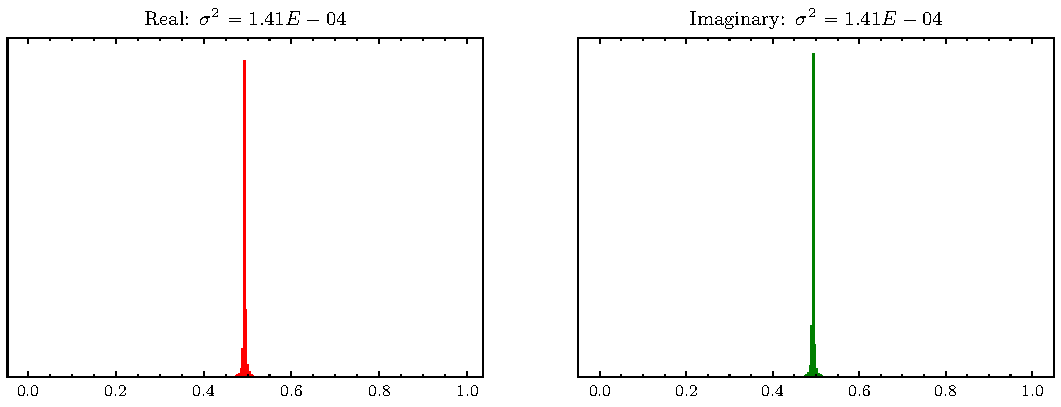
\includegraphics[width=.9\textwidth]{cost2100_indoor_sph_dist.pdf}
	\medskip
	\caption{Distribution and variance of COST2100 real/imaginary channels under spherical normalization ($N=99000$) images.}
	\label{fig:cost_indoor_sph_dist}
\end{figure}

Beyond desirable properties in the input distribution, spherical normalization also results in an objective function which is better matched with the evaluation criterion. Neural networks for CSI estimation are optimized using the mean-squared error loss,
\begin{align} 
	\text{MSE}&=\frac 1N \sum_{k=1}^N\Arrowvert\mathbf H_k - \hat{\mathbf H}_k\Arrowvert^2, \label{eq:mse}
\end{align}
while channel state reconstruction accuracy is measured in terms of normalized mean-squared error,
\begin{align} 
	\text{NMSE}&=\frac 1N \sum_{k=1}^N\frac{\Arrowvert\mathbf H_k - \hat{\mathbf H}_k\Arrowvert^2}{\Arrowvert\mathbf H_k\Arrowvert^2}. \label{eq:nmse}
\end{align}
Observe that when the $\mathbf H_k \; (\hat{\mathbf H}_k)$ in (\ref{eq:mse}) is replaced with $\check{\mathbf H}_k \; (\hat{\check{\mathbf H}}_k)$, we have
\begin{align*} 
	\frac 1N \sum_{k=1}^N\Arrowvert\check{\mathbf H}_k - \hat{\check{\mathbf H}}_k\Arrowvert^2&= \frac 1N \sum_{k=1}^N\left\Arrowvert \frac{\mathbf H_k}{\Arrowvert\mathbf H_k\Arrowvert^2} - \frac{\hat{\mathbf H}_k}{\Arrowvert\mathbf H_k\Arrowvert^2}\right\Arrowvert^2 \\
	&= \frac 1N \sum_{k=1}^N\frac{\Arrowvert\mathbf H_k - \hat{\mathbf H}_k\Arrowvert^2}{\Arrowvert\mathbf H_k\Arrowvert^2},
\end{align*}
which is equivalent to (\ref{eq:nmse}). Thus, a neural network optimized with MSE as the loss function and trained using spherically normalized data is in fact being optimized with respect to NMSE of the original data.

\subsection{Results}
Training on spherically normalized data and optimizing with respect to NMSE can yield better accuracy. Fig.~\ref{fig:nmse_slot1} demonstrates this improvement for CsiNet and CsiNet Pro on the COST2100 dataset. For both networks, the number of 

\begin{figure}[!hbtp] \centering 
	\begin{subfigure}[t]{.45\textwidth}
		\centering
		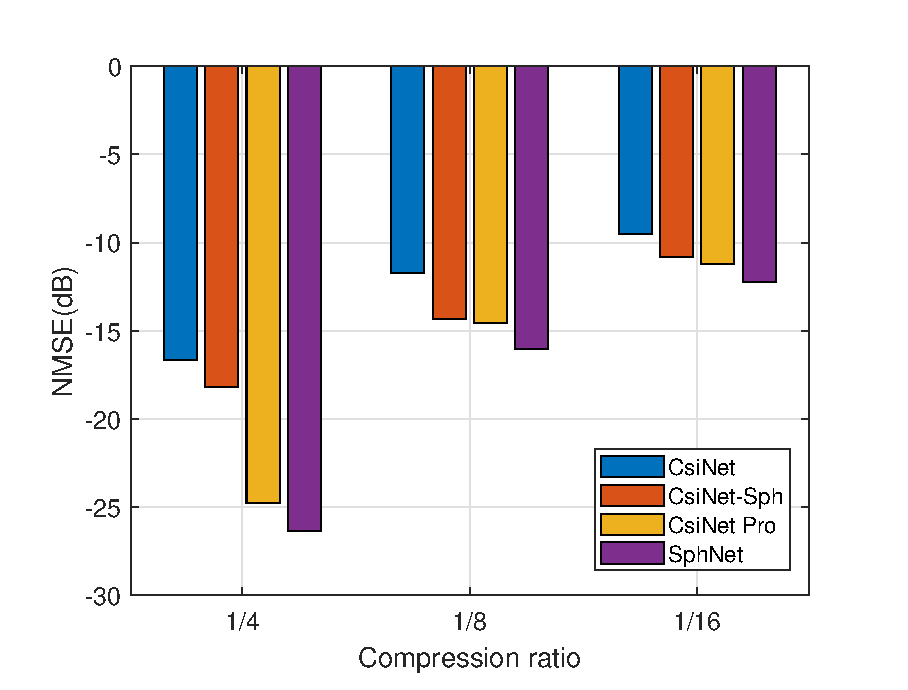
\includegraphics[width=\linewidth]{nmse_slot1_indoor.eps}
		\caption{Indoor}
		\label{fig:slot1_indoor} 
	\end{subfigure}
	\begin{subfigure}[t]{.45\textwidth}
		\centering
		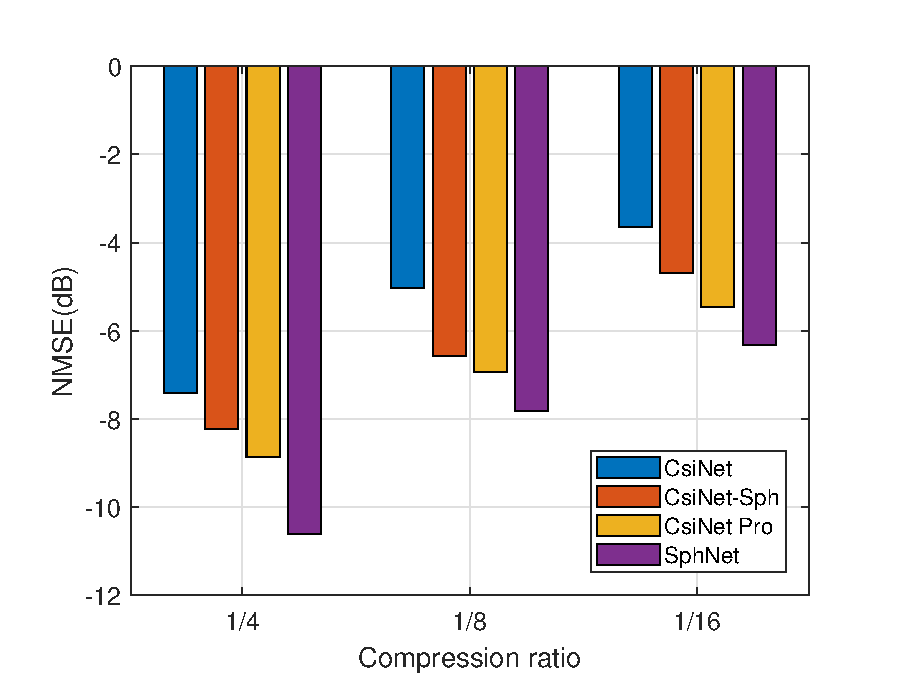
\includegraphics[width=\linewidth]{nmse_slot1_outdoor.eps}
		\caption{Outdoor}
		\label{fig:slot1_outdoor} 
	\end{subfigure}
	\caption{Reconstruction error for CsiNet \cite{ref:csinet} and CsiNet Pro with and without spherical normalization. SphNet combines CsiNet Pro with spherical normalization \cite{ref:liu2020sphnet}.}
	\label{fig:nmse_slot1} 
\end{figure}


\section{MarkovNet: A Deep Learning-based Differential Autoencoder}
\label{chap:previous_2}
% 03_markovnet.tex
In this section, we consider methods for exploiting temporal correlation between CSI of subsequent timeslots.
Assuming the channel coherence within a certain window of time,
a reasonably accurate CSI estimate at time $t-1$ can be used to estimate the CSI at time $t$.
Generically, we can write this estimator as
\begin{align}
\grave{\mathbf H}_t &= h(\hat{\mathbf H}_{t-1}) \label{eq:gen_estim}
\end{align}
where $\mathbf{H}_t$ is the CSI matrix at time $t$ and $\hat{\mathbf H}_t$ is its estimator. 
The estimation error under $\grave{\mathbf H}_t$ is
\begin{align}
\mathbf E_{t} &= \mathbf H_{t} - \grave{\mathbf H}_{t}. \label{eq:diff_err}
\end{align}

\subsection{Related Work}

Prior work in temporal correlation for CSI estimation utilized state-space methods such as the Kalman filter \cite{ref:Huber2006improved,ref:Ali2020BayesKalmanFilter,ref:Kim2021KalmanVsML}. Since it relies on explicit state space and noise models, the Kalman filter's predictive power in CSI estimation is limited. Furthermore, such work generally does not propose a method for feedback compression, making comparison with the following ML methods difficult.

Recent works have leveraged recurrent neural networks (RNNs) to exploit temporal correlation for CSI estimation \cite{ref:Lu2019RecCsiNet, ref:Liao2019BiLSTM, ref:Li2020SpatTempLSTM,
 ref:Jang2019Delay,ref:Wang2019CsiNetLSTM}. RNNs include recurrent layers, such as the long short-term memory (LSTM) cell or the gated recurrent unit (GRU), which are capable of learning long-term dependencies of a given process through backpropagation \cite{ref:Hermans2013Training} and can be used to predict future states of the process \cite{ref:Pascanu2014HowTo}.

\begin{figure}[htb]
	\centering
	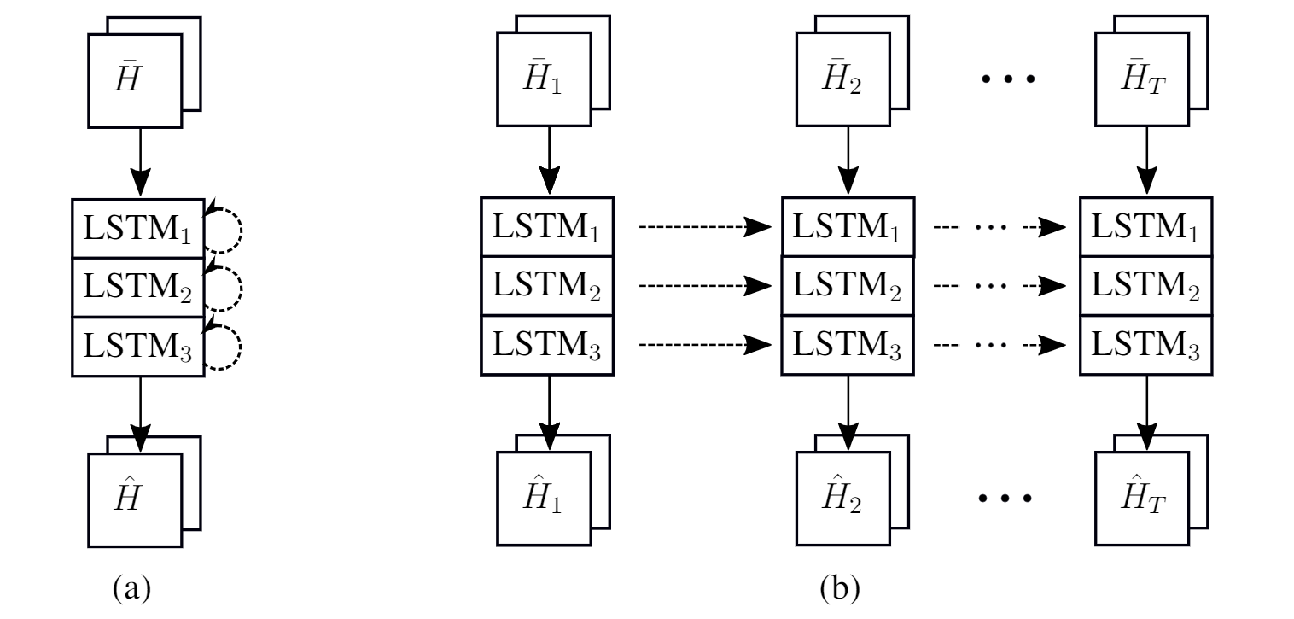
\includegraphics[width=.9\textwidth]{lstm-example-unroll.pdf}
	\medskip
	\caption{An example of LSTMs used for CSI estimation. (a) ``Stacked'' LSTM network of depth 3 shown with recurrent connections. (b) Same LSTM network ``unrolled" into $T$ timeslots }
	\label{fig:lstm_example}
\end{figure}

RNNs have been used extensively in natural language processing (NLP) for machine translation \cite{ref:Sutskever2014seq2seq} and sentiment extraction \cite{ref:Irsoy2014opinion}. For such works in NLP, authors have empirically found ``stacked'' or ``deep'' RNNs to be effective (e.g., Fig.~\ref{fig:lstm_example}), hypothesizing that having multiple recurrent layers allows the network to extract different semantic timescales \cite{ref:Irsoy2014opinion, ref:Bengio2009Learning}. Works in CSI estimation have taken cues from this work in NLP, proposing CSI estimation networks with stacked LSTMs after a sequence of autoencoders \cite{ref:Wang2019CsiNetLSTM}. While such work has demonstrated the utility of RNNs, the computational cost of LSTMs can be prohibitively high. For example, the RNN portion of the network proposed in \cite{ref:Wang2019CsiNetLSTM} accounts for $10^8$ additional parameters. Since channel estimation should not place an undue computational burden on the communications system, LSTMs can be problematic.

\subsection{Methods}

Rather than use RNNs to extract temporal dependencies in CSI data, we proposed a lightweight network based on the principle of differential encoding. We trained a network to estimate the error (\ref{eq:diff_err}) under a linear estimator, 
\begin{align*}
	\grave{\mathbf H}_t &=  \hat{\mathbf H}_{t-1} \mathbf W
\end{align*}
where $\mathbf W \in \mathbb C^{R_b \times R_b}$ is the minimum mean squared error (MMSE) estimator.
\begin{align*}
	\mathbf H_t &= \mathbf H_{t-1}\mathbf W + \mathbf E_t \\
	\mathbf H_{t-1}^H\mathbf H_t &= \mathbf H_{t-1}^H\mathbf H_{t-1} \mathbf W + \mathbf H_{t-1}^H\mathbf E_t
\end{align*}
Under the principle of orthogonality, the error term $\mathbf E_t$ is orthogonal with the observed data, and the product $\mathbf H^H_{t-1}\mathbf E_t$ becomes a zero matrix. Denoting the cross correlation matrix as $\mathbf R_{i} = \mathbb{E}\left[\mathbf H_{t-i}^H\mathbf H_{t}\right]$.
\begin{align*}
	\mathbf W &= \mathbf R_0^{-1} \mathbf R_1 
\end{align*}
In practice, the population correlation matrices are estimated
via finite samples of size $N$,
\begin{align*}
	\mathbf{\hat R}_i &= \frac 1N \sum_{j}^N \mathbf H_{t-i}^H(j)\mathbf H_{t}(j),
\end{align*}
where $\mathbf H_t(j)$ is the $j$-th sample in the training set.
The MMSE estimator based on the sample correlation matrices is written as
\begin{align*}
	\hat{\mathbf W} &= \hat{\mathbf R}_0^{-1} \hat{\mathbf R}_1.
\end{align*}
We can further simplify this estimator to a scalar, $\gamma \in \mathbb R$, as
% \begin{align*}
%   \hat \gamma &= \frac{\sum_{i=1}^N\text{Trace}(\left[\mathbf H_{t-1}^H(i)\mathbf H_{t}(i)\right])}{\sum_{i=1}^N\Arrowvert\mathbf H_t^H(i) \mathbf H_t(i)\Arrowvert^2},
% \end{align*}
\begin{align*}
	\hat \gamma &= \frac{\text{Trace}(\hat{\mathbf R}_1(k,l))}{\sum_k^{R_d}\sum_l^{N_b}\hat{\mathbf R}_0(k,l)},
\end{align*}
where $k$ ($l$) are the row (column) indices of the correlation matrices. The estimator in this case is 
\begin{align}
	\grave{\mathbf H}_t &= \hat\gamma \hat{\mathbf H}_{t-1} \label{eq:gamma-estim}.
\end{align}
Under the estimator $\gamma$, we proposed to encode the error, $\mathbf E_t$, using a convolutional autoencoder, $f(\mathbf E_t)$,
\begin{align*}
	\hat{\mathbf E}_t &= g(f(\mathbf E_t, \vec\theta_e), \vec\theta_d),
\end{align*}
where $\mathbf E_t = \mathbf H_t - \gamma\hat{\mathbf H}_{t-1}$. The base station has access to the estimators $\gamma$ and $\hat{\mathbf H}_{t-1}$, and the resulting CSI estimate at $t$ is
\begin{align}
	\hat{\mathbf H}_t &= \hat\gamma \hat{\mathbf H}_{t-1} + \hat{\mathbf{E}}_t \label{eq:diff-estim}
\end{align}

\subsubsection{MarkovNet}

In \cite{ref:Liu2020MarkovNet}, we proposed MarkovNet, a deep differential autoencoder. Each timeslot of MarkovNet uses an instance of CsiNet-Pro with unique parameters. The network at the first timeslot ($t_1$) is trained directly on the CSI ($\mathbf H_1$). For all subsequent timeslots, $t_i$ for $i \geq 2$, we use the MMSE estimator (\ref{eq:gamma-estim}) to produce an error term $\mathbf E_t$, and the autoencoder in each timeslot is trained to produce an error estimate, $\hat{\mathbf E}_t$. The estimated error is added back per (\ref{eq:diff-estim}) to produce a refined estimate.

\begin{figure}[!hbtp]
    \centering
    {
      \fontsize{6pt}{8pt}
      \def\svgwidth{0.8\columnwidth}
      \input{../images/markovnet_schematic.pdf_tex}
    }
    \caption{Abstract architecture for MarkovNet. Networks at $t_i$ for $i \geq 2$ are trained to predict the estimation error, $\mathbf E_i$.}
    \label{fig:markovnet_schema}
\end{figure}

The resulting network requires no recurrent layers, resulting in a substantial reduction in computational complexity. Table~\ref{tab:comp-complex} shows the number of parameters and FLOPs per timeslot for CsiNet-LSTM, MarkovNet, and CsiNet. The parameter count of MarkovNet is on par with CsiNet, and CsiNet-LSTM requires orders of magnitude more parameters. While the number of FLOPs for MarkovNet is nearly 10 times smaller than CsiNet-LSTM, MarkovNet requires 5 to 10 times more FLOPs than CsiNet due to the increased kernel size of CsiNet-Pro.

\begin{table}[htb]
  \renewcommand{\arraystretch}{1}
  \begin{center}
  % \caption{Table II: Model size \& computational complexity comparison. M: million, K: thousand.}
  \caption{Model size/computational complexity of tested temporal networks (CsiNet-LSTM, MarkovNet) and comparable non-temporal network (CsiNet). M: million.}
  \label{tab:comp-complex} 
  % \resizebox{\linewidth}{15mm}
  \footnotesize{
	  \begin{tabular}{|l|c|c|c|c|c|c|}
	  \hline
	                              & \multicolumn{3}{c|}{\textbf{Parameters}} & \multicolumn{3}{c|}{\textbf{FLOPs}} \\ \hline
	                              & \textbf{CsiNet-LSTM} & \textbf{MarkovNet} & \textbf{CsiNet} & \textbf{CsiNet-LSTM} & \textbf{MarkovNet} & \textbf{CsiNet} \\ \hline
	  \textbf{CR=$1/4$}  		  & 132.7 M              & 2.1 M              & 2.1 M  			& 412.9 M              & 44.5 M             & 7.8 M           \\ \hline
	  \textbf{CR=$1/8$}  		  & 123.2 M              & 1.1 M              & 1.1 M  			& 410.8 M              & 42.	4 M             & 5.7 M           \\ \hline
	  \textbf{CR=$1/16$} 		  & 118.5 M              & 0.5 M              & 0.5 M 			& 409.8 M              & 41.3 M             & 4.7 M           \\ \hline
	  \textbf{CR=$1/32$} 		  & 116.1 M              & 0.3 M              & 0.3 M           & 409.2 M              & 40.8 M             & 4.1 M           \\ \hline
	  \textbf{CR=$1/64$} 		  & 115.0 M              & 0.1 M              & 0.1 M 			& 409.0 M              & 40.5 M             & 3.9 M           \\ \hline
	  \end{tabular}
  }
  \end{center}
\end{table} 

\subsection{Numerical Results}

We compare MarkovNet with CsiNet-LSTM \cite{ref:Wang2019CsiNetLSTM} on the indoor and outdoor COST2100 datasets (for details, see Section~\ref{sect:channel_model}). For MarkovNet, we train the network at the first timeslot for 1000 epochs. In each subsequent timeslot, we initialize the network using the weights from the previous timeslot and train for 200 epochs. We use a batch size of 200. We perform a training/testing split of 75k/25k samples, and we estimate $\gamma$ using the training set. To compare the estimation accuracy of each network, we report the NMSE.
%estimate of the previous timeslot with the scalar MMSE estimator, $\gamma$, to produce the error term $\mathbf E_t = \mathbf H_t - \gamma\hat{\mathbf H}_{t-1}$.

Figure~\ref{fig:diffnet_result} shows the NMSE of MarkovNet and CsiNet-LSTM for four different compression ratios. For the indoor network, all instances of MarkovNet achieve lower NMSE than all instances of CsiNet-LSTM. In the outdoor scenario, each CR for MarkovNet demonstrates lower NMSE than the corresponding CR for CsiNet-LSTM. Between both channel scenarios, MarkovNet shows gradual improvement for subsequent timeslots if the CR is high enough while CsiNet-LSTM only improves gradually in the outdoor environment for CR$=\frac 14$.
\begin{figure}[!hbtp] \centering 
	\begin{subfigure}[t]{.45\textwidth}
		\centering
		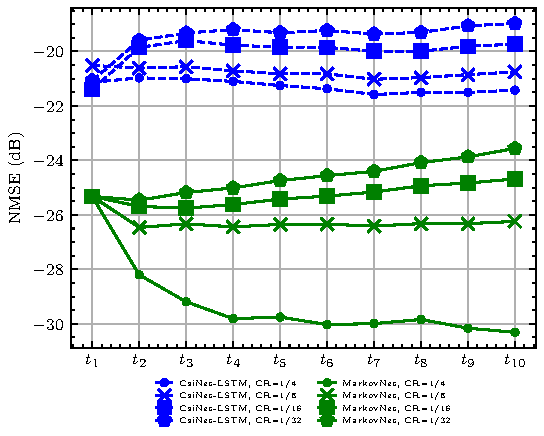
\includegraphics[width=\linewidth]{MarkovNet_truncated_Indoor_10slots.pdf}
		\caption{Indoor}
		\label{fig:diffnet_indoor} 
	\end{subfigure}
	\begin{subfigure}[t]{.45\textwidth}
		\centering
		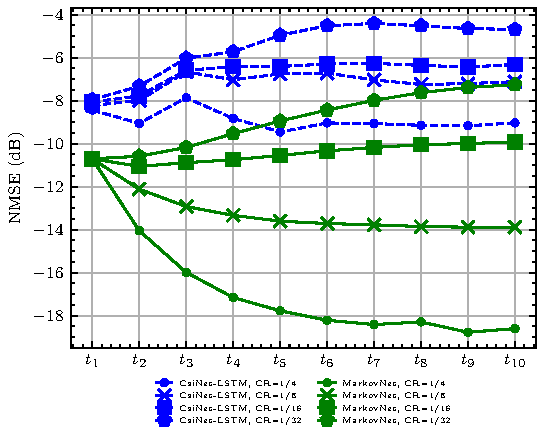
\includegraphics[width=\linewidth]{MarkovNet_truncated_Outdoor_10slots.pdf}
		\caption{Outdoor}
		\label{fig:diffnet_outdoor} 
	\end{subfigure}
	\caption{$\text{NMSE}$ comparison of MarkovNet and CsiNet-LSTM 
	at various compression ratios (CR).} 
	\label{fig:diffnet_result} \vspace*{-2mm}
\end{figure}  
Figure~\ref{fig:csi_image} shows a random sample from the test set, $\mathbf H$, and the estimates produced by CsiNet-LSTM and MarkovNet for a CR of $\frac 14$. This sample contains three ``peak'' magnitude regions. While both networks manage to capture the two larger samples, MarkovNet is able to recover the small peak magnitude region ({\color{darkgreen}green arrow}) which CsiNet-LSTM fails to produce ({\color{red}red arrow}).

\begin{figure}[htb] \centering 
	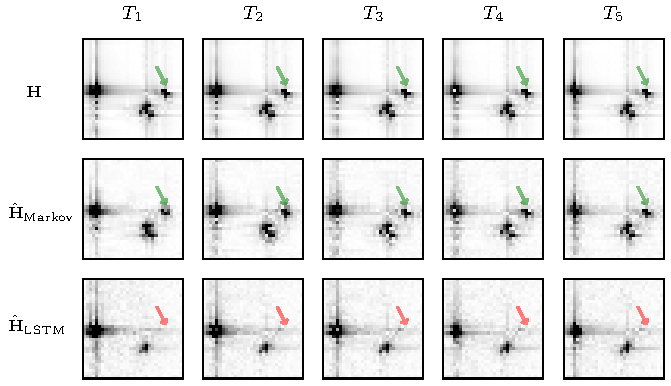
\includegraphics[width=0.9\linewidth]{batch0_csi_compare_cr512_annot.pdf}
	\caption{CSI ($\mathbf H$), MarkovNet estimates ($\hat{\mathbf H}_{\text{Markov}}$), and CsiNet-LSTM estimates ($\hat{\mathbf H}_{\text{LSTM}}$) across five timeslots ($T_1$ through $T_5$) on one outdoor channel sample from the test set,
using $\text{CR}=\frac 14$.} 
	\label{fig:csi_image} 
\end{figure}

\section{Proposed Work}
\label{chap:proposed}
% 04_proposed_work.tex

\subsection{Proposed Work Section \#1}

\subsubsection{Proposed Work Subsection \#1}
\blindtext

\subsubsection{Proposed Work Subsection \#2}
\blindtext
\blindtext


\section{Conclusion}
% 05_conclusion.tex

In this proposal, we discussed techniques for efficient MIMO channel state information (CSI) estimation. We outlined the author's prior work using spherical normalization, which scales each CSI sample by its power, and a deep learning framework for differential encoding, which exploits temporal correlation between CSI at subsequent timeslots. We outlined a future research effort in soft-to-hard vector quantization for practical CSI feedback compression, and we presented initial results based on the SHVQ framework for this network.

\newpage
\small
\bibliographystyle{ieeetr}
\bibliography{../cited_works}

\end{document}